\chapter{Theoretische Grundlagen}

\section{Verbraucher in Inselnetzen}

Der folgende Abschnitt befasst sich mit der Beschreibung der Stromverbraucher für das vorliegende Inselnetz. 
Für eine fiktive Kommune gibt es verschiedene Verbrauchertypen, welche es näher zu untersuchen gilt. 
Ziel dabei ist es, reale Verbraucher zu kategorisieren und ihren Verlauf genauer zu analysieren. 
Da der Fokus der Simulation auf dem Netz und Speichertechnologien liegt, werden Vereinfachungen zur Darstellung in MatLab/Simulink vorgenommen.
Die Betrachtung potentieller Verbraucher und ihre Modellierung in einem Inselnetz-Modell wird in den folgenden beiden Abschnitten genauer analysiert. 
Im ersten Schritt wird die momentane Situation in Deutschland und seinen Kommunen hinsichtlich Differenzierung und Verbrauch beschrieben. 
Danach erfolgt die Ermittlung eines Konzepts zur Abschätzung von Verbräuchen mittels Lastkurven. 
Ziel der Unterteilung ist zuerst einen Überblick über die Basis des zu modellierenden Inselnetzes zu schaffen. 
Danach gilt es daraus pauschale Verbräuche unter Einbezug von Lastkurven zu ermitteln, welche in MatLab/Simulink simulationstauglich sind.

\subsection{Verbraucher am Stromnetz}

Die potentiell zu betrachtenden Verbraucher für das Inselnetz entsprechen dabei denen einer deutschen Kommune am deutschen Stromnetz. 
Sie werden dabei in verschiedene Kategorien unterteilt und in folgenden Sub-Abschnitten genauer analysiert. 
Dabei erfolgt eine Differenzierung in Wohngebäude (WG), Nichtwohngebäude (NWG), die Interaktion dieser beiden Verbraucher mit eigenen Speichern, Windkraft und PV-Anlagen im Unterpunkt „Prosumer“, der Faktor Elektromobilität und weitere Verbraucher, die noch nicht betrachtet wurden. 
Die für das Inselnetz relevanten Parameter sind hierbei der Stromverbrauch und das Lastprofil jeden Verbrauchers, sowie deren Vorkommen in einer durchschnittlichen, deutschen Kommune. 
Außerdem wird noch die Möglichkeit der Einspeisung von Strom in ein Fernwärmenetz bzw. die Umwandlung von Strom in Wasserstoff als Power-to-Gas beschrieben.

\subsubsection{Wohngebäude (WG)}

In Deutschland gibt es etwa 19,5 Mio. Wohngebäude, die an das Stromnetz angebunden sind. Dabei hat jedes Wohngebäude einen Energieverbrauch, der sich aus verschiedenen Faktoren zusammensetzt. 
Diese lassen sich in Raumwärme, Warmwasser, Beleuchtung, Betrieb von Elektrogeräten und sonstiger Prozesswärme unterteilen. 

\begin{figure}[h!]
    \centering
    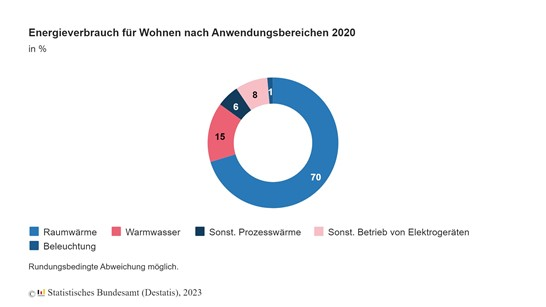
\includegraphics[width=14cm]{Abbildungen/VerbraucherAbb1.jpg}
    \caption{Energieverbrauch WG\cite{destatisenergie]}\label{fig:Energieverbrauch_WG}
\end{figure}

Hierbei werden die Faktoren Elektrogeräte und Beleuchtung in der Regel durch Strom gedeckt. 
Die Faktoren Warmwasser und Raumwärme sind abhängig vom eingebauten Heizungssystem. 
Hierbei sind eine anteilige bis vollständige Erzeugung der Raumwärme und des Warmwassers durch eine strombetriebene Wärmepumpe, eine Stromheizung oder ein Wärmenetz möglich und für die Simulation relevant. 
Dabei ist zu beachten, dass insbesondere bei Wärmepumpen der Wärmeenergieverbrauch stark vom Strombedarf abweicht. 
Eine Umrechnung mit Hilfe der Jahresarbeitszahl (JAZ) ist möglich. 
Im Neubau liegt der Anteil der verbauten Wärmepumpen im Jahr 2022 bei ca. 57\%.

Die Höhe des Energieverbrauches ist außerdem abhängig von der Anzahl der Bewohner des Wohngebäudes und dessen Größe als auch Zustand. 
Im Gebiet Wohnen und Gebäude werden daher viele Annahmen und Hochrechnungen pro Kopf, pro Fläche oder pro Haushalt getätigt. Um die Verbraucher für verschiedene Simulationsszenarien vereinfacht zu ermitteln, wird hier wie im Folgenden beschrieben vorgegangen. 

\begin{figure}[h!]
    \centering
    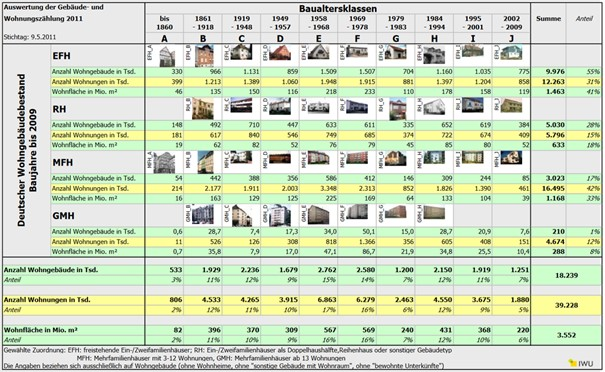
\includegraphics[width=14cm]{Abbildungen/VerbraucherAbb2.jpg}
    \caption{Deutscher Wohngebäudebestand\cite{baualtersklassen}}\label{fig:Deutscher_Wohngebäudebestand}
\end{figure}

Wohngebäude lassen sich generell noch in weitere Unterkategorien aufgliedern.
Dazu zählen Einfamilienhäuser, Mehrfamilienhäuser, große Mehrfamilienhäuser, Reihenhäuser, Hochhäuser und Doppelhaushälfte, sowie diverse Spezialfälle. 
Um die Simulation der Verbraucher simpel zu halten, werden zum Verbraucher „Einfamilienhaus“ auch energetisch in der gleichen Größenordnung liegende Wohngebäudetypen gezählt, beispielsweise Reihen- und Zweifamilienhäuser. 
Der Verbraucher „Mehrfamilienhaus“ umfasst äquivalent auch solche Wohngebäudetypen. 
Große Mehrfamilienhäuser (ab 13 Wohnungen), Hochhäuser und mittelgroße bis große Wohnheime werden in der Praxis dazugezählt. 
Diese werden nicht in der Simulation dargestellt.
Das liegt einerseits daran, dass es sich nicht um eine großstädtische Simulation handelt, andererseits daran, dass bei außergewöhnlich großen Wohngebäuden individuell stark abweichende Energieverbräuche – auch beim Stromverbrauch – entstehen. 
Der Einbezug dieser übersteigt die Komplexität dieses Aspektes der Simulation.
Unter Einbezug des Heizungssystems gilt es einen Gesamtenergieverbrauch des Verbrauchers zu ermitteln. 
Der Jahresverbrauch von Wohnenergie liegt pro Einfamilienhaus bei etwa 25.000 kWh. 
Mehrfamilienhäuser sind meist energieeffizienter was den Heizenergieverbrauch betrifft, jedoch hängt der Verbrauch stark von der Anzahl der Wohnfläche, Wohnungseinheiten und Bewohnern ab. 
Aus Simplifizierungsgründen wird hier mit dem bundesweiten Jahresenergieverbrauch pro Kopf gerechnet, 8.800 kWh. 
Bei der Annahme von durchschnittlich 12 Personen pro Mehrfamilienhaus entspricht dies einem Jahresenergieverbrauch von 105.600 kWh. 
Es wird angenommen, dass der Anteil vom Energieverbrauch sich zu 85\% auf das Heizen bezieht. 
Wenn man nun davon ausgeht, dass entweder eine Wärmepumpe oder ein anderes Heizungssystem verbaut ist, welches nicht auf Strom basiert, ergeben sich vier Szenarien. 
Bevor jedoch ein Stromverbrauch bei Nutzung einer Wärmepumpe errechnet werden kann, ist zu beachten, dass der Energieverbrauch durch den Wirkungsgrad der Wärmepumpe in Stromverbrauch umgerechnet werden muss. 
Dies über die Jahresarbeitszahl JAZ möglich. 
Bei dem am meisten verbauten Typ von Wärmepumpen, den Luft-Wasser-Wärmepumpen, liegt dieser üblicherweise im Bereich von 2 bis 4. 
Für die Berechnung wird mit einer JAZ von 3 gerechnet. Daher ergibt sich folgende Formel:

\begin{equation}
    \text{Strom pro Jahr} = \text{Enrg. pro Jahr} \times \frac{0.85}{3} + \text{Enrg. pro Jahr} \times 0.15
\end{equation}

Liegt keine Wärmepumpenheizung vor, wird der erste Teil des Terms gleich null gesetzt. 
Die vier resultierenden Verbrauchertypen werden in nachfolgender Tabelle aufgeführt, wobei aufgerundet wird:

\begin{table}[htbp]
    \centering
    \caption{4 Szenarien (exakter Wert in den Klammern)}
    \label{tab:szenarien}
    \begin{tabular}{lccc}
        \toprule
        \textbf{Szenario/Verbrauch [kWh/a]} & \textbf{Einfamilienhaus} & \textbf{Mehrfamilienhaus} \\
        \midrule
        Heizung Wärmepumpe & 7,000 (7,083) & 30,000 (29,920) \\
        Heizung nicht abgebildet & 3,750 & 16,000 (15,840) \\
        \bottomrule
    \end{tabular}
\end{table}

Der Momentanverbrauch wird durch Lastprofile abgeschätzt und im entsprechenden Abschnitt bearbeitet.

\subsubsection{Nichtwohngebäude (NWG)}

Die Anzahl an Nichtwohngebäuden beläuft sich auf 21,5 Mio. in Deutschland, von denen 6 Mio. thermisch konditioniert sind. 
Diese lassen sich allgemein in Dienstleistungsgebäude, beispielsweise Schulen, Büros, Gastro, Sport und Produktionsgebäude, beispielsweise Werkstätten, Lager, Betriebe, unterteilen. 
Der Energieverbrauch allgemein und einhergehend der Stromverbrauch ist hierbei stark nutzungsabhängig. 
Während sich bei Dienstleistungsgebäuden die Verbrauchsfaktoren meist noch anteilig ähnlich derer bei Wohngebäuden verhalten, ist dies bei Produktionsgebäuden nicht der Fall. 
Dies geht soweit, dass eine Pauschalisierung der Verbrauchsaufschlüsselung nicht möglich ist.

\begin{figure}[h!]
    \centering
    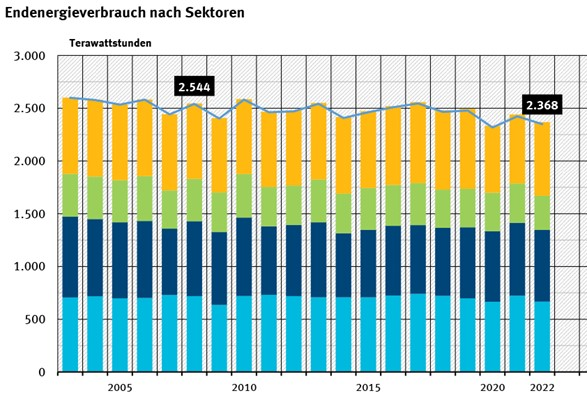
\includegraphics[width=14cm]{Abbildungen/VerbraucherAbb3.jpg}
    \caption{Endenergieverbrauch nach Sektoren\cite{uwb}}\label{fig:Endenergieverbrauch_nach_Sektoren}
\end{figure}

Trotz deutschlandweit bekannter Gesamtverbräuche ist der Energiebedarf in einer Kommune stark von lokalen Gewerbegebieten und einzelnen Großverbrauchern abhängig. 
Diese sind für eine Simulation individuell abzuschätzen. Die Stromverbrauchsabschätzung ist dabei hauptsächlich produktabhängig und bedarf branchenüblicher Kennzahlen.

\subsubsection{Elektromobilität}

Im Abschnitt Elektromobilität als Verbraucher gilt es den Stromverbrauch durch Elektromobilität, also vorwiegend E-Autos zu bestimmen. 
Diese kann dann einem bereits bekannten Verbraucher zuzuordnen ist, z.B. einem Einfamilienhaus oder einzeln oder zu mehreren (Bsp. Tankstelle) betrachtet werden.
Mögliche Nutzer einer E-Ladesäule sind E-Autos, E-Motorräder und E-Bikes. 
Um ein einfaches Modell zu erhalten, werden alle Nutzer einer E-Zapfsäule als E-Autos betrachtet, da diese absolut und verbrauchsmäßig der größte Nutzer sind. 
Für private E-Zapfsäulen bietet es sich an, über gefahrene Kilometer und Verbrauch eine pauschale Abschätzung zu treffen. 
Pro E-Auto kommt man bei den durchschnittlich gefahrenen 15.000 km pro Jahr auf einen Verbrauch von 2.250 kWh Strom. 
Bei anderen E-Zapfsäulen ist auch eine Abschätzung in E-Auto-Jahresstromverbräuchen sinnig. 
Da diese nicht mit einem privaten Speicher interagieren, wie bei privaten E-Zapfsäulen, lassen sich diese einfach zusammenfassen.

\subsubsection{Prosumer: Gebäude mit PV/Windkraft/Speicher}

Als private Speicher, Windkraft und PV sind hier ebensolche gemeint, die einem WG oder NWG konkret zugeordnet werden können und keine eigenständigen, kommerziellen Anlagen sind. 
Diese sind keine eigenen Verbraucher, aber ein Faktor bei der Findung von Verbrauchszahlen von den genutzten WG und NWG als auch der Elektromobilität.
Die beschriebenen PV-Anlagen sind für die Simulation hinsichtlich ihrer Höchstleistung, in kWp angegeben, relevant. 
Bei Einfamilienhäusern liegt diese meist im Bereich von 15-25 kWp, bei Mehrfamilienhäusern von 20 bis zu 40 kWp und im Bereich der NWG bis zu 99 kWp. 
Da bei NWG häufig große Dachflächen zur Verfügung stehen, werden entsprechend 99 kWp installiert. 
Aufgrund von gesetzlichen Vorschriften im Rahmen des GEG’s sind größer dimensionierte Anlagen die Ausnahme.
Windkraft im privaten Bereich ist in den letzten Jahren immer relevanter geworden. 
Die Stromerzeugung liegt bei bis zu 1 kWh/a pro Haushalt. 
Da diese sie noch nicht als wirtschaftlich gelten und bei der Stromerzeugung eine nicht-relevante Rolle spielen, wird sie in dieser Simulation nicht betrachtet.
Private Stromspeicher werden üblicherweise in Verbindung mit Eigenerzeugung von Strom durch PV installiert. 
Stand heute besitzen 12\% der Haushalte eine PV, jedoch besitzt nur jeder dritte einen dazugehörigen Stromspeicher. 
Eine Dimensionierung des Speichers erfolgt in Abhängigkeit zur kWp der eigenen PV-Anlage. 
Eine Faustformel ist hierbei pro 1 kWp Höchstleistung 1kWh Speicher zu dimensionieren. 
Bei Nutzung der Mittelwerte für die Dimensionierung von PV-Anlagen pro Verbraucher der Faustformel zur Speicherdimensionierung ergeben sich folgende Werte:

\begin{table}[htbp]
    \centering
    \caption{Dimensionierung}
    \label{tab:dimensionierung}
    \begin{tabular}{lccc}
        \toprule
        \textbf{Szenario} & \textbf{Einfamilienhaus} & \textbf{Mehrfamilienhaus} & \textbf{NWG} \\
        \midrule
        PV [kWp] & 20 & 30 & 99 \\
        Stromspeicher [kWh] & 20 & 30 & 99 \\
        \bottomrule
    \end{tabular}
\end{table}

\subsubsection{Weitere Verbraucher}

Für eine Kommune als Inselnetz gibt es noch zwei weitere Verbraucher, dessen Einfluss in einem Inselnetz geprüft werden muss. 
Dabei handelt es sich um Eisenbahn, ein Wärmenetz und Straßenbeleuchtung.
Die Eisenbahn in Deutschland wird i.d.R. durch das Bahnstromnetz versorgt, dessen Betrachtung außerhalb eines kommunalen Inselnetzes liegen würde. 
Ein Bahnstromnetz wird daher nicht simuliert.
Der letzte zu betrachtende Verbraucher ist die Straßenbeleuchtung. 
Generell ist diese schwierig zu betrachten, da Verbräuche kommunal stark schwanken. 
Dies hat damit zu tun, dass die Dichte an Straßenlaternen, als auch die genutzte Technik im Verbrauch starke Unterschiede aufweist. 
Statistisch liegt der Stromverbrauch der Straßenbeleuchtung bei 40 bis 80 kWh pro Einwohner pro Jahr. 
Es ist erwähnenswert, dass der Anschluss der Straßenbeleuchtung meist über separate Beleuchtungskabel erfolgt.

\subsubsection{Umwandlung in Fernwärme/Power-to-Gas (Wasserstoff)}

Die Umwandlung in Wärme und Verteilung durch ein Fernwärmenetz ist eine mögliche Option zur Energieversorgung. 
Ein solches kann der Simulation beigefügt werden und ist ein Spezialfall. 
Der Bedarf an Wärmeenergie, welche relevant für die Simulation ist, wenn sie durch Strom erzeugt wird, ist gekoppelt an Endverbraucher, z.B. Einfamilienhäuser. 
Jedoch bringt ein Fernwärmenetz flexible Speichermöglichkeiten für Erzeugungsspitzen mit sich. 
So kann das Fernwärmenetz über den Energiebedarf der Endverbraucher erhitzt werden und dabei Energie in Form von Wärme zwischenspeichern. 
Die Dimensionierung dieses Netzes ist abhängig von der Anzahl der Verbraucher, dessen Wärmebedarf aus oberen Abschnitten bereits bekannt ist. 
Der Wirkungsgrad liegt bei 80 – 90\%.
Bei Power-to-Gas handelt es sich um eine ähnliche Methode. 
Da der Wasserstoff in Speichern, statt in einem Netz gespeichert werden kann, ist die Nutzung flexibler und sogar der Export möglich. 
Der Strom-zu-Strom-Wirkungsgrad, also inklusive der Umwandlung von Gas-to-Power, liegt bei etwa 70\%.

\subsection{Verbrauchsermittlung auf Basis von Lastkurven}

Lastkurven dienen in der Elektrizitätswirtschaft dazu, den prognostizierten Strombedarf für verschiedene Verbraucher im Stromnetz abzuschätzen. 
Diese Unterscheidung erfolgt zeitlich in 15-Minuten-Schritten. 
Dazu kommt zusätzlich eine saisonale und tagesbezogene Unterteilung. 
Die Simulation des Strombedarfs in einem Inselnetz wird für einen diskreten Zeitpunkt benötigt und lässt sich mit Hilfe der Lastkurven beschreiben. 
Der Bezug und die Verarbeitung der Daten aus zugänglichen Lastprofilen werden zunächst genauer beschrieben. 
Weitere notwendige Schritte zur Implementierung und Nutzung der Daten bei Zeitschritten unter 15 Minuten.
Für die verschiedenen Verbraucher gibt es eine größere Anzahl an unterschiedlichen Lastprofilen. 
Da der Fokus der Simulation auf Speichertechnologien liegt, ist es sinnvoll, ähnliche Lastkurven zusammenzufassen und auf den Endverbrauch hin zu skalieren. 
Die Auswahl und Zusammenfassung der vorhandenen Lastkurven kann folgender Tabelle entnommen werden. 
Als Kriterium für die Nutzung gilt der Anteil in einer Kommune, die auf Basis erneuerbarer Energien ihre Stromversorgung gewährleistet.

\begin{table}[htbp]
    \centering
    \caption{Liste verfügbare Lastprofile}
    \label{tab:lastprofile}
    \begin{tabular}{llcc}
        \toprule
        \textbf{Bezeichnung} & \textbf{Beschreibung} & \textbf{Nutzung} & \textbf{Quelle} \\
        \midrule
        H0 & Haushalt & Ja & VDEW (SLP) \\
        G0 & Gewerbe allgemein & Nein & VDEW (SLP) \\
        G1 & Gewerbe werktags 8-18 Uhr & Nein & VDEW (SLP) \\
        G2 & Gewerbe mit starkem Verbrauch in den Abendstunden & Nein & VDEW (SLP) \\
        G3 & Gewerbe durchlaufend & Nein & VDEW (SLP) \\
        G4 & Laden/Friseur & Ja & VDEW (SLP) \\
        G5 & Bäckerei mit Backstube & Ja & VDEW (SLP) \\
        G6 & Wochenendbetrieb & Nein & VDEW (SLP) \\
        L0 & Landwirtschaftsbetriebe & Ja & VDEW (SLP) \\
        L1 & Landwirtschaftsbetriebe mit Nebenerwerb/-zucht & Nein & VDEW (SLP) \\
        L2 & Übrige Landwirtschaftsbetriebe & Nein & VDEW (SLP) \\
        W0 & Wärmepumpen & Ja & SWKiel Netz GmbH \\
        N0 & Nachtspeicherheizungen & Nein & SWKiel Netz GmbH \\
        24h & 24h-Band & Nein & SWKiel Netz GmbH \\
        T0 & Telefonzellen & Nein & SWKiel Netz GmbH \\
        A0 & Ampelanalgen & Ja & SWKiel Netz GmbH \\
        S0 & Straßenbeleuchtung & Ja & SWKiel Netz GmbH \\
        B1 & BHKW mit KWK & Nein & SWKiel Netz GmbH \\
        B2 & BHKW ohne KWK & Nein & SWKiel Netz GmbH \\
        \bottomrule
    \end{tabular}
\end{table}

Aufgrund ähnlicher Lastkurven von den Lastprofilen G0 bis G6 erfolgt eine vereinfachte Aufteilung des Gewerbes auf die sich deutlich unterscheidenden Lastprofile G4 und G5.
G0, G1 und G3 werden dabei in G4 betrachtet und G2 in G5. 
G6 fällt unter L0. 
Alle Landwirtschaftsbetriebe sind außerdem pauschal über L0 berücksichtigt. 
Aufgrund der vereinfachten Annahme, dass alle Haushalte, die ihre Heizenergie über das Stromnetz beziehen, eine Wärmepumpe nutzen, wird W0 mit der Bedingung W0≤H0 genutzt, da davon ausgegangen wird, dass pro Haushalt maximal eine Wärmepumpe genutzt wird. 
Es ist anzumerken, dass im Lastprofile H0 der Strombedarf für Raumwärme und Warmwasser nicht berücksichtigt ist. 
BHKW’s stellen als zu simulierendes Objekt eine große Herausforderung dar und werden daher auch nicht betrachtet.
Die Angaben von Lastprofilen erfolgt in 15-Minuten-Schritten in der Einheit Watt als Leistungswerte für den Jahresverbrauch von 1.000kWh. 
Bei einer Simulationsschrittgröße ab 1 Sekunde sind daher Leistungswerte pro Sekunde notwendig. 
Es müssen daher zwei Schritte vorgenommen werden. 
Es bedarf einer Skalierung des Jahresverbrauches pro Einheit und einen „Momentanverbrauch“ für jeden Simulationsschritt.
Die Jahresverbräuche wurden im Abschnitt „Verbraucher am Stromnetz“ abgeschätzt und können übernommen werden. 
Für Landwirtschaftliche- und gewerbliche Verbraucher unterscheidet sich der Verbrauch stark durch Flächen- und Produktionsunterschiede. 
Daher wurden Schätzfaktoren im Verhältnis zum Haushalt aufgestellt. Die genutzten Faktoren können folgender Tabelle entnommen werden.

\begin{table}[htbp]
    \centering
    \caption{Skalierungsfaktor Lastprofile Jahresverbrauch}
    \label{tab:skalierungsfaktor}
    \begin{tabular}{lcl}
        \toprule
        \textbf{Lastprofil} & \textbf{Faktor zum Jahresverbrauch (1000 kW * Faktor)} \\
        \midrule
        H0 & 7* \\
        G4 & 20 \\
        G5 & 50 \\
        L0 & 30 \\
        W0 & 10*\\
        A0 & 1 \\
        S0 & 1 \\
        \bottomrule
    \end{tabular}
\end{table}
*auf Basis des Verhältnisses von EFH und MFH nach Verbrauchswerten aus Tabelle Dimensionierung berechnet
    
Der Jahresverbrauch einer Straßenlaterne ist bei Nutzung von LEDs bei etwa 168 kWh. 
Aus Simplifizierungsgründen wird mit dem Faktor 1 gearbeitet, also entspricht eine Einheit einem Zug von 6 Straßenlaternen. 
Bei Ampelanlagen hängt dies von der Größe und Anzahl Leuchtfelder, als auch der genutzten Technik, ab. 
Der jährliche Durchschnittsverbrauch liegt bei 1.600 kWh , jedoch sind Ampelanlagen im nicht innerstädtischen Bereich meist weniger in Nutzung und deutlich kleiner. 
Daher wird mit einem Verbrauch von 1.000 kWh simuliert. Die Anzahl an Einheiten ist nun mit einem weiteren Skalierungsfaktor wählbar.
Die Betrachtung vom Strombedarf in 1-Sekunden statt 15-Minuten-Schritten kann durch Interpolation erreicht werden. 
Hierbei lassen sich alle Werte sekündlich abschätzen, wodurch ein Momentanverbrauch, welcher für die Simulation des Stroms im Netz und der genutzten Speichertechnologien wichtig ist, simulierbar ist. 
Die Interpolation kann direkt in MatLab/Simulink durch sogenannte Look-Up-Tables durchgeführt werden.
 
\begin{figure}[h!]
    \centering
    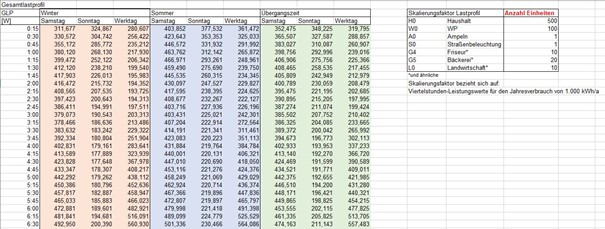
\includegraphics[width=14cm]{Abbildungen/VerbraucherAbb4.jpg}
    \caption{Excel-Tool zu Erstellung und Skalierung von Gesamtlastprofilen (eigene Darstellung)}\label{fig:Excel-Tool_zu_Erstellung_und_Skalierung_von_Gesamtlastprofilen}
\end{figure}

Zur Erstellung von zu importierenden Last- bzw. Gesamtlastprofilen steht ein selbstgebautes Excel-Tool zur Verfügung. 
Dieses bietet die Möglichkeit, Skalierungs- und Einheitenfaktoren für die hinterlegten Lastprofile anzupassen. 
Ein resultierendes Lastprofil wird ausgegeben und kann direkt in entsprechende Look-Up-Tables des Simulationsaufbaus importiert werden.

\section{Stabilität in Inselnetzen}

Ein Zentrales Kriterium bei der Auslegung und dem betrieb von elektrischen Energiesystemen stellt die Stabilität dar. Durch sie wird eine lückenlose und zuverlässige Stromversorgung gewährt. Die Stabilität in Energiesystemen definiert sich daraus, wie ein System auf Störeinflüsse oder Änderungen im Last- oder Erzeugungsverhalten reagiert. Die verschiedenen Stabilitätskriterien lassen sich wie  \autoref{fig:stabil} zeigt in verschiedene Kategorien klassifizieren. 

\begin{figure}[H]
	\centering
	\includegraphics[width=0.8\linewidth]{Abbildungen/Stabilität.png}
	\caption{Klassifizierung der Stabilität in Inselnetzen nach}
	\label{fig:stabil}
\end{figure}

Grundsätzlich ergeben sich hieraus drei Stabilitätsbetrachtungen, die im Folgenden kurz erläutert werden. Obwohl sich das Modell in \autoref{fig:stabil} lediglich mit der Frequenzstabilität beschäftigt, werden der Vollständigkeit halber und für das allgemeine Verständnis auch die anderen beiden Stabilitätskriterien kurz umrissen.

\textbf{Frequenzstabilität}

Die Frequenzstabilität beschreibt Phänomene, welche sich aus der Wirkleistungsbilanz des Netzes ergeben. 
Die Frequenz hängt direkt mit dem Gleichgewicht aus Erzeugung und Verbrauch von Wirkleistung zusammen, 
weshalb diese auch ein Maß für die ausgeglichene Bilanz in einem Energiesystem darstellt. 
Die Arten der Störungen werden hierbei noch in ihre Dauer und ihren Einfluss auf das System kategorisiert. 
Ein Ausfall einer kleinen Erzeugungsanlage stellt beispielsweise eine Kleinstörung dar, welche durch eine 
geeignete Regelung der Erzeugungsanlagen auch schnell wieder ausgeregelt werden kann. 
Ein Kurzschluss stellt wiederum eine Großstörung dar, welche sich bei einem korrekten Verhalten der 
Schutztechnik schnell auflöst aber auch bei einem ungewollten Verhalten langfristig anhalten kann. 
Besonders in kleineren Inselnetzen wirken sich der Ausfall einer Erzeugunsganlage stärker aus als in 
einem großen Verbundnetz mit relativ großer Trägheit. Hinzu kommt die mangelnde Trägheit der Generatoren 
bei einer Erzeugung aus erneuerbaren Erzeugungsanlagen, welche meistens über Wechselrichter an das Netz 
gekoppelt sind. \cite{Simulationsmethoden} Zudem besteht in Inselnetzen durch die geringe Ausddehnung eine 
hohes R/X-Verhältnis, welches zu einer Kopplung zwischen Spannungs- und Frequenzstabilität führt. 
Denn eine Spannungsänderung an der Erzeugungsanlage wirkt sich unmittlebar auf den verbraucher aus, 
weelcher druch die geringere Spannung zusätzlich eine geringere Leistung abruft. \cite{Willenberg2021}

\textbf{Spannungsstabilität}

Die Spannungsstabiltät beschreibt das Verhalten der Spannungen in allen Knoten des Netzes un dist im 
wesentlichen von der Blindleistungsbilanz abhängig. In Inselnetzen spielt diese aber meistens eine 
untergeordnete Rolle, da der Blindleistungsbedarf aufgrund der geringen Ausdehnung und damit verbundenen 
kleinen Übertragungsleitungen relativ gerin gausfällt. Viel wichtiger ist hier die richtige Aufteilung der 
Blindleistungserzeugung auf die Erzugungsanlagen, da bei unvporteilhafter AUfteilung hohe Blindströme fließnen, 
welche sich wiederrum auf die Spannungsstabilität auswirken. Falls die Erzeugungsanlagen einen erhöhten 
Blindleistunsgbedarf durch z.B. eine Störung nicht ausregeln, wirkt sich dies besonders Stark auf die 
Spannung im Netz aus. Jedoch wird der Spannungsstabilität aufgrund des begrenzten Umfangs in den folgenden 
Modellen keine Betrachtung geschenkt.

\textbf{Regelungssystems}

Durch die hohe Dezentralität der Erzeugungsanlagen und dem Verzicht auf große Kraftwerke ist eine optimale 
Regelung der Erzeugungsanlagen unter Betrachtung der oben genannten Kriterien notwendig. 
Elektrische Maschienne bilden durech ihre Massenträgheit eine gewisse Trägheit in der Asuwirkung von 
Störungen oder Disbalancen und stabilisieren das Netzsomit von selbst. In Wechselrichtergeführten Netzen 
könenen sich besonders durch die Schaltfrequenzen der Leistungselektronik gegenseitige Beeinflussungen der 
Erzeugungsanlagen bilden. Daher stellt die Regelung dieser System eine besondere Herausforderung dar. 
Die Regelung des System wird jedoch aufgrund der Oberflächliche nBetrachtung ebenfalls im weiteren verlauf 
vernachlässigt.



\section{Speichertechnologien in Inselnetzen}

\subsection{Gründe für den Einsatz von Speichern in Inselnetzen}
Für diese Projektarbeit soll ein autarkes Inselnetz mit regenerativer Energieerzeugung 
modelliert und simuliert werden.
Aus verschiedenen Gründen, welche im Folgenden genauer erläutert werden sollen, ist der Einsatz von
Speichertechnologien für die Umsetzung eines solchen Inselnetzes zwingend notwendig.

Grundlegend ist eine lückenlose Energieversorgung innerhalb eines Netzes nur möglich wenn nahezu gleich viel Energie in das Netz
eingespeist und abgenommen wird.
Entscheidende Parameter für die Regelung der Energieerzeugung sind dabei vor Allem die Netzfrequenz 
und -spannung.
Das deutsche Verbundnetz ist dafür in vier Regelzonen unterteilt, welche wiederrum in verschiedene
Bilanzkreise unterteilt sind.
Innerhalb dieser Bilanzkreise wird anhand von Voraussagen für den nächsten Tag versucht
eingespeiste und entnommene Leistung auszuregeln.
Durch den schwankenden Leistungsbedarf sind Abweichungen hier allerdings die Regel.
Bei der Betrachtung eines regenerativen Inselnetzes kommt die volatile Natur von regenerativen Energieerzeugern
als weiterer Faktor hinzu und erschwert eine korrekte Voraussage enorm.
Diese Abweichungen der tatsächlich benötigten Leistung von der bereitgestellten führen zu Frequenzschwankungen
welche sich wiederrum negativ auf die Netzstabilität auswirken.
Zum Ausgleich dieser Schwankungen muss Regelenergie zur Verfügung gestellt werden.

\begin{figure}[h!]
    \centering
    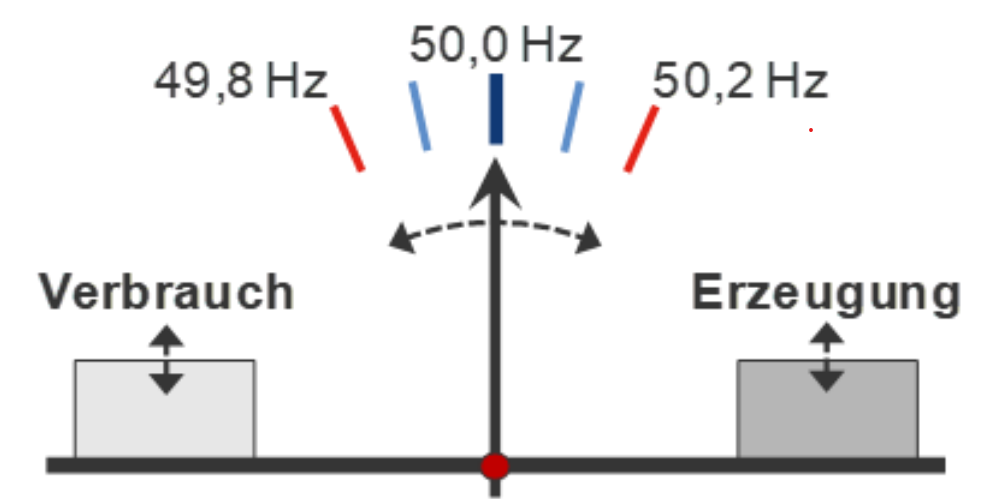
\includegraphics[width=6cm]{Abbildungen/Sollfrequenz.png}
    \caption{Frequenzschwankungen durch Ungleichgewicht von erzeugter und verbrauchter Leistung~\parencite{cronenberg_beschreibung_nodate}}\label{Gleichgewicht}
\end{figure}

Die benötigte Energie ist dabei unterteilt in Momentanreserve, Primärreserve, Sekundärreserve 
und Tertiärreserve.
Die Momentanreserve, welche geringe Frequenzabweichung direkt ausgleichen soll, wird im deutschen Verbundnetz
durch die Schwungmasse der Kraftwerks-Synchronmaschinen bereit gestellt.
Die Primärreserve hingegen greift erst ab einer Abweichung von $20\ mHz$ und muss nach spätestens 30 Sekunden
sowie für mindestens 15 Minuten vollständig zur Verfügung stehen.
Hierfür werden heute schon zunehmend Batteriespeicher eingesetzt.
Zusätzlich wird nach 30 Sekunden die Sekundärregelleistung bereit gestellt, welche für eine Stunde verfügbar sein muss.
Nach 15 Minuten wird diese dann von der Tertiärregelreserve abgelöst, welche ebenfalls für eine Stunde verfügbar sein muss.
Die beiden letzten Regelenergie-Kategorien werden in aller Regel von Kraftwerken in Teillast oder Kraftwerken mit kurzen Anfahrzeiten
erzeugt.
Zuletzt werden einzelne Netzabschnitte vom Netz getrennt um einen Zusammenbruch des Bilanzkreises zu vermeiden.
Dieses Vorgehen bleibt allerdings die äußerste Maßnahme und soll in aller Regel vermieden werden.

Für ein Inselnetz besteht nicht die Möglichkeit Teilnetze abzutrennen. 
Im schlimmsten Fall müssen einzelne Verbraucher und Erzeuger vom Netz getrennt werden um einen stabilen Betrieb zu sichern.
Um das weitestgehend zu vermeiden, ist eine Überdimensionierung von Erzeugern und Speichern meist das Mittel der Wahl.
Große Speicher zur Primärreserve bilden dabei einen wichtigen Grundpfeiler, wobei gerade Batteriespeicher 
auf Grund ihres schnellen Regelverhaltens in Frage kommen~\parencite{Itschner}.

Zusätzlich sollen hier neben der klassischen Regelreserve der Vollständigkeit halber die Regelleistungsprodukte \texttt{Enhanced Frequency Response}
(EFR) und \texttt{Virtuelle Schwungmasse} (VSM) erwähnt werden.
Diese sind zwar noch nicht in den deutschen Markt integriert, könnten aber in der Zukunft eine wichtige Rolle spielen.

EFR setzt dabei schon vor der Primärreserve ein und stellt die volle Regelenergie ab spätestens 1 Sekunde bereit.
Damit füllt EFR die Lücke die durch die fehlenden großen Synchronmaschinen entsteht und wird z.B. bereits vom 
größten britischen Netzbetreiber eingesetzt.
Durch die hohen Anforderungen an die Einschaltzeiten bieten sich auch für diesen Einsatz vor allem
Lithium-Ionen-Batterien an~\parencite{mantar_gundogdu_battery_2018}.

Beim Prinzip der VSM wird versucht die Frequenzstabilität zu verbessern indem Speicher an das Netz angeschlossen werden
die im Wesentlichen das Trägheitsverhalten von mechanischen Schwungmassen in Generatoren imitieren.
Gerade kleiner Inselnetzen welche vor allem durch regenerative Energien betrieben werden könnten hierdurch profitieren.
Auf Grund des kontinuierlichen Energieaustausches mit dem Netz bieten sich für die Umsetzung von VSM-Anlagen vor allem
Speicher mit hoher Lebensdauer und Zyklenzahl an~\parencite{boxleitner_virtuelle_2009}.

\subsection{Rahmenbedingung und Bestimmungen}

In Deutschland sind die Übertragungsnetzbetreiber dafür verantwortlich die Frequenz innerhalb ihrer Regelzone auf möglichst
50 Hz zuhalten.
Dafür stehen Ihnen die oben genannten Regelreserveprodukte zur Verfügung, welche von unterschiedlichen Teilnehmern
des Regelreservemarktes bereit gestellt werden können.
Die verschiedenen Übertragungsnetzbetreiber kooperieren dabei im Netzregelverbund, welcher ein Konzept darstellt,
die Vorhaltung von Regelreserve technisch und wirtschaftlich zu optimieren.
In Zukunft ist ein solches, stark koordiniertes Vorgehen auch auf zentraleuropäischer Ebene geplant.

Im Folgenden sollen die Anforderungen und Bestimmungen zu den einzelnen in Deutschland zugelassenen Regelreserveprodukten 
zusammengefasst werden.

\begin{itemize}
    \item Primärreserve oder \texttt{Frequency Containment Reserve} (FCR) ist darauf ausgelegt die Netzfrequenz möglichst schnell zu stabilisieren. Dafür wird die FCR proportional zur Abweichung der Frequenz von ihrem Sollwert geregelt. Sie wird automatisch bei Abweichungen über 10 mHz aktiviert und soll spätestens nach 30 Sekunden vollständig zur Verfügung stehen.
    \item Sekundärreserve oder \texttt{automatic Frequency Restoration Reserves} (aFRR) löst die Primärreserve ab indem sie die Frequenzabweichung vollständig ausgleicht. Die aFRR ist dafür als Proportional-Integral-Regelung umgesetzt und ist nicht nur abhängig von der Netzfrequenzabweichung sondern zusätzlich vom Leistungsaustausch zwischen den Bilanzkreisen.
    \item Tertiärreserve oder \texttt{manual Frequency Restoration Reserve} (mFRR) löst die aFRR bei länger anhaltenden Störungen ab. Sie ist daher nicht automatisch aktiviert und muss erst innerhalb von 15 Minuten vollständig aktivierbar sein.
\end{itemize}

Zusätzlich sind in \parencite[]{Verordnung} folgende FCR-spezifischen Anforderungen genannt:
\begin{itemize}
    \item [\glqq{} a] die FCR-Aktivierung darf nicht künstlich verzögert werden und muss nach einer Frequenzabweichung so bald wie möglich beginnen;
    \item [b] im Falle einer Frequenzabweichung von mindestens 200 mHz sind spätestens nach 15 Sekunden mindestens 50 \% der vollständigen FCR-Kapazität bereitzustellen;
    \item [c] im Falle einer Frequenzabweichung von mindestens 200 mHz sind spätestens nach 30 Sekunden 100 \% der vollständigen FCR-Kapazität bereitzustellen;
    \item [d] im Falle einer Frequenzabweichung von mindestens 200 mHz muss die Aktivierung der vollständigen FCR-Kapazität im Intervall von 15 bis 30 Sekunden mindestens linear ansteigen, und 
    \item [e] im Falle einer Frequenzabweichung von weniger als 200 mHz muss die entsprechende aktivierte FCR-Kapazität mindestens proportional zu dem unter den Buchstaben a bis d genannten gleichen Zeitverhalten sein.\grqq{}
\end{itemize}

\begin{figure}[h!]
    \centering
    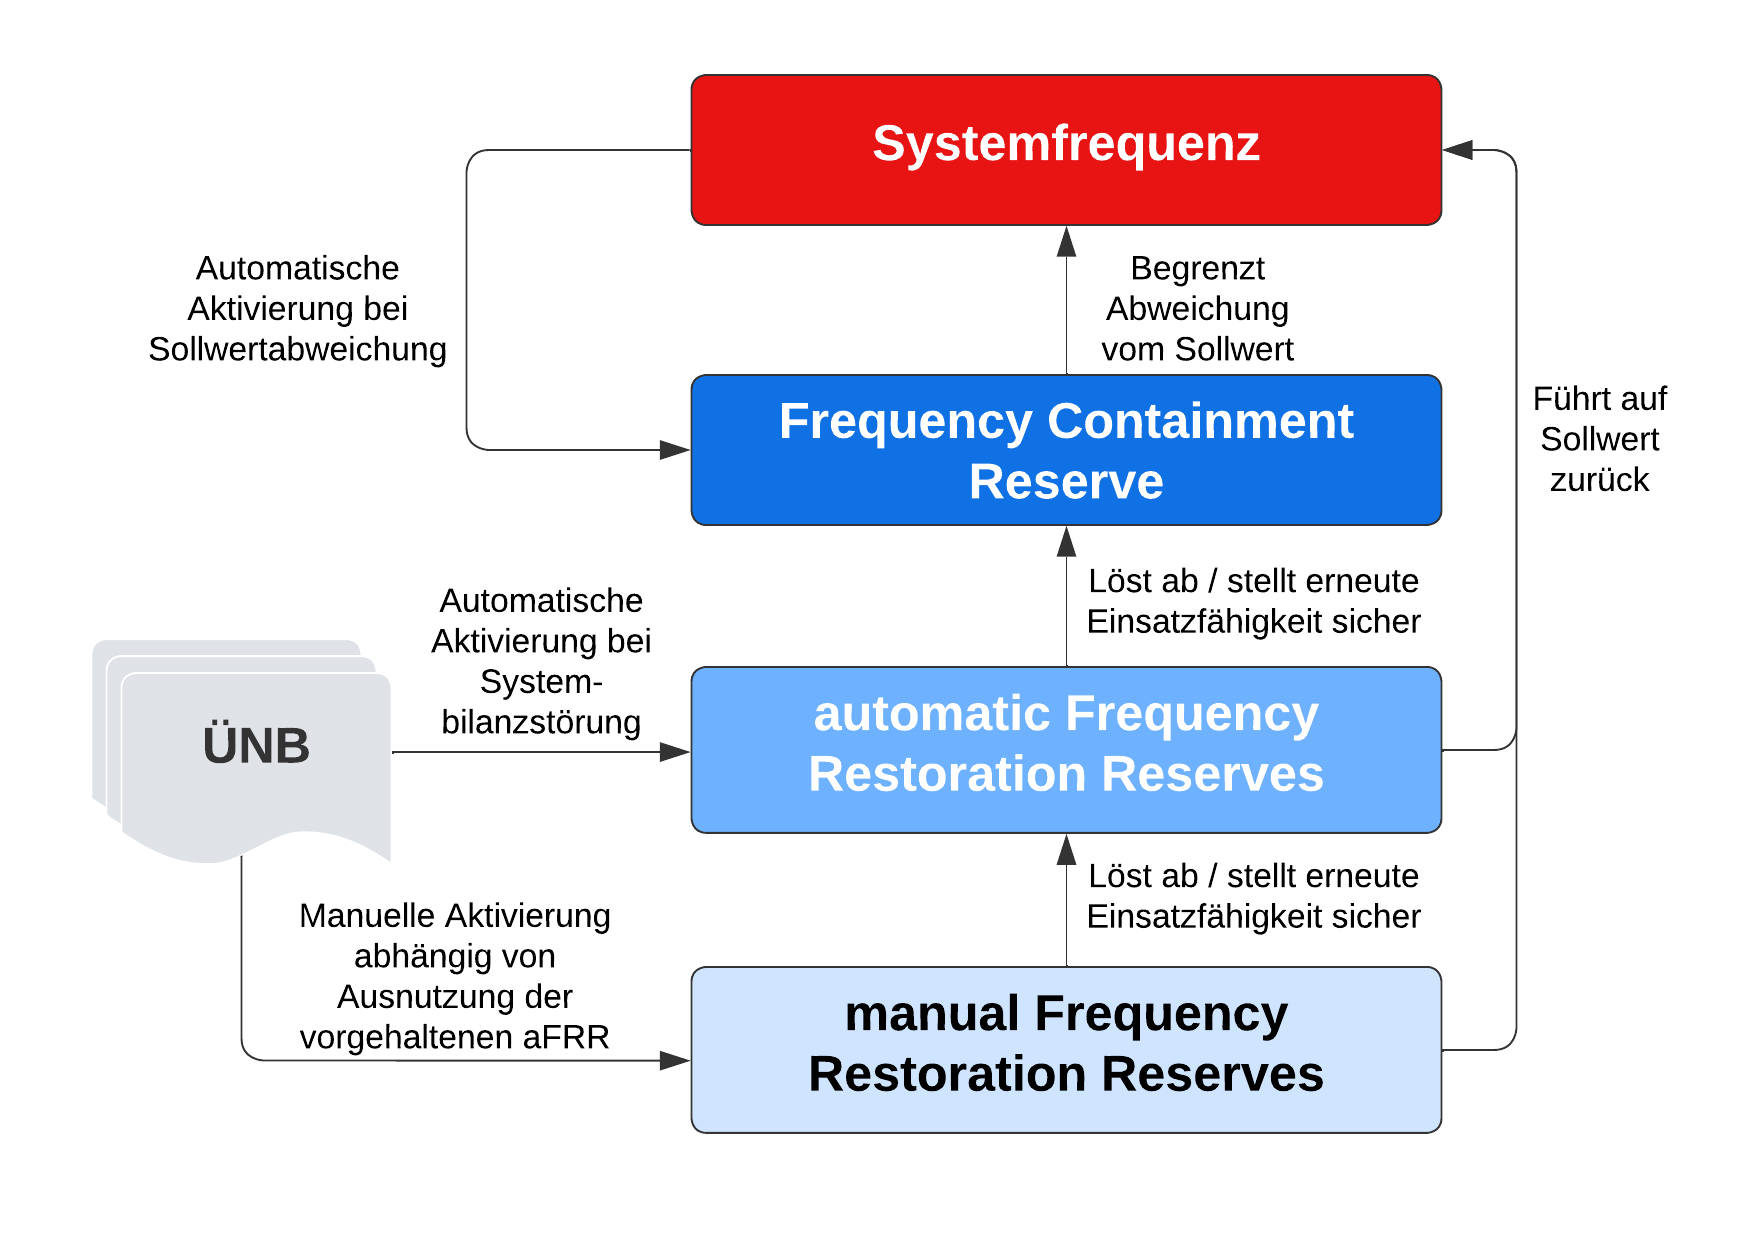
\includegraphics[width=11cm]{Abbildungen/_Flussdiagramm (1).png}
    \caption{Überblick über die verschiedenen Regelreserveprodukte aus~\parencite{cronenberg_beschreibung_nodate}}\label{Fluss}
\end{figure}


\subsection{Betriebsstrategien zu Batteriespeichern}\label{Betriebsstrategien}

Für die Modelle und Simulationen in dieser Projektarbeit werden von den, im letzten Paragraphen beschriebenen Regelreserveprodukten
im Wesentlich zwei genauer betrachtet.
Einerseits die Primärreserve oder FCR und andererseits die EFR, die zwar bisher von deutschen Übertragungsnetzbetreibern nicht genutzt wird
aber gerade für ein Inselnetz wie das hier geplante, eindeutige Vorteile bietet.

Betrachtet man die Anforderungen an diese beide Methoden der Regelleistungsbereitstellung, so kommen vor allem
Batteriespeicher und insbesondere Lithium-Ionen-Batterien für eine Auswahl der Speichertechnologien in Frage.
Im Folgenden sollen verschiedene Methoden zur Umsetzung von FCR- und EFR-Speichern mit Hilfe von Batteriespeichern 
diskutiert und vorgestellt werden.

Beim Betrieb von Batteriespeichern zur Bereitstellung von Regelleistung ist der limitierende Faktor der Kapazitäten zu bedenken.
Durch den so genannten State of Charge (SOC) kann ausgedrückt werden, wie viel Prozent ihrer Kapazität einer Batterie noch zur Verfügung stehen.
Um möglichst zu jedem Zeitpunkt die Anforderungen an die PCR oder EFR erfüllen zu können ist eine intelligente
SOC-Steuerung daher unerlässlich.

\begin{figure}[h!]
    \centering
    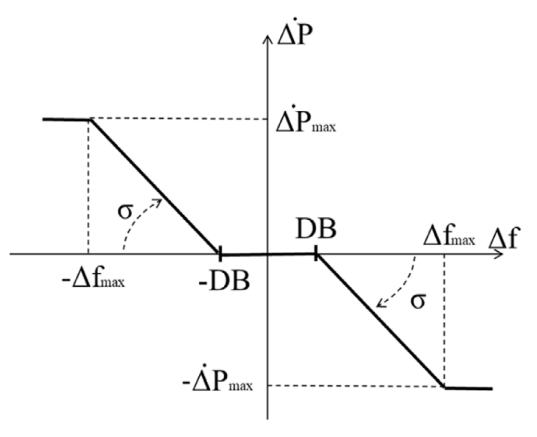
\includegraphics[width=8cm]{Abbildungen/DroopControl.png}
    \caption{Vorgabe der Leistungskurve für PCR-Bereitstellung aus~\parencite[Kap. 3]{noauthor_soc_nodate}}\label{Droop}
\end{figure}

Abbildung~\ref{Droop} zeigt den vorgegebenen Verlauf der Leistungsbereitstellung für PCR-Produkte.
Im letzten Paragraphen wurde bereits beschrieben, dass hierbei ein proportionaler Verlauf zur Frequenzabweichung 
gefordert ist, sobald die Abweichung einen gewissen Grenzwert überschreitet.
Bei einer reinen Umsetzung dieser Kurve mit Hilfe von Batterien, würde unweigerlich, ein Ungleichgewicht von 
Frequenzerhöhungen und Frequenzeinbrüchen dazu führen, dass die Batteriespeicher irgendwann keine Leistung mehr
zur Verfügung stellen können.

Um das zu vermeiden wird in~\parencite[]{noauthor_soc_nodate} unter anderem eine sogenannte Dead band strategy beschrieben.
Der Grundgedanke sieht vor, dass ein Ziel-SOC von z.B. 50 \% festgelegt wird und anschließend während Phasen mit 
Frequenzabweichung innerhalb der Grenzwerte Leistung ausgetauscht werden kann, um den optimalen SOC zu erreichen.
Die maximale Leistung die dabei genutzt werden darf, ist in Deutschland beschränkt.
So darf über 50 Hz keine Leistungsabgabe mehr erfolgen und unter 50 Hz keine Leistungsaufnahme,
sofern allerdings innerhalb des Totbandes dem linearen Verlauf der Leistungskurve gefolgt wird,
ist ein Leistungsaustausch zulässig~\parencite[]{marchgraber_modellierung_2019}.

\begin{figure}[h!]
    \centering
    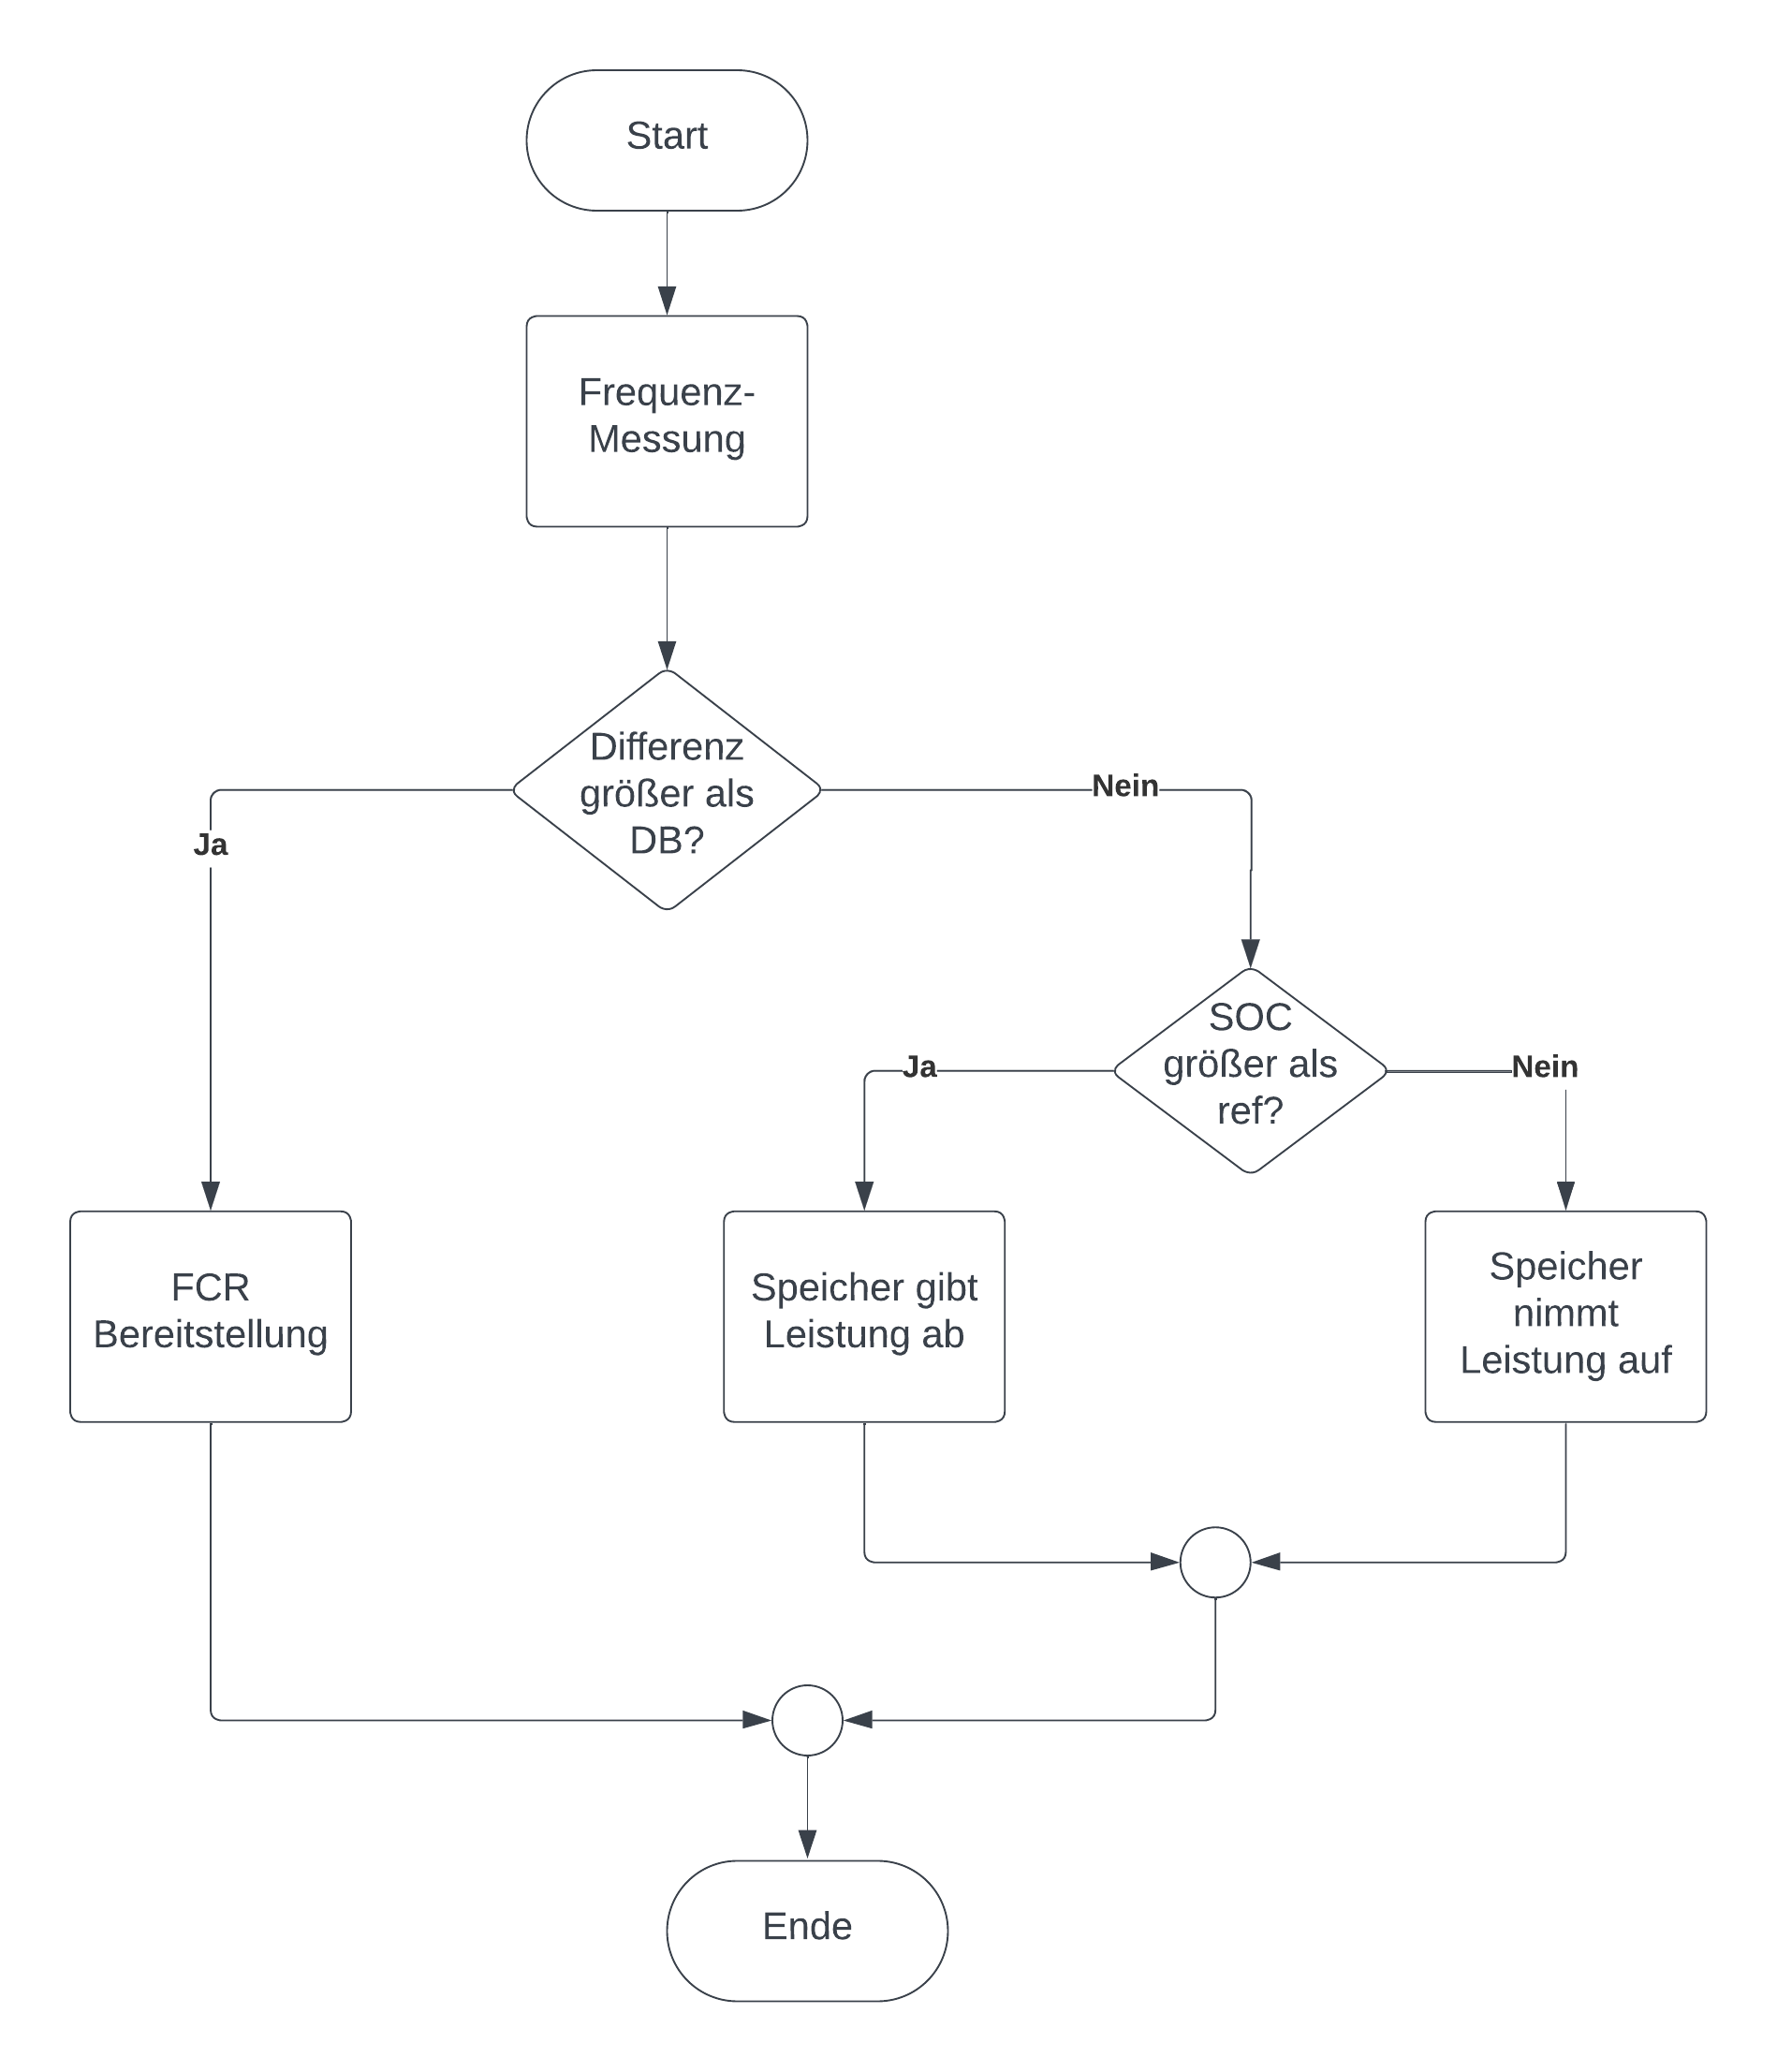
\includegraphics[width=8cm]{Abbildungen/DBFlow.png}
    \caption{Flussdiagramm zur Deadband-Strategie nach~\parencite[]{noauthor_soc_nodate}}\label{FlowPCR}
\end{figure}

Abbildung~\ref{FlowPCR} zeigt ein Flussdiagramm zur Ausnutzung des Totbandes.
Ein Nachteil dieser Methode bleibt allerdings, dass nur bei geringen Abweichungen der Netzfrequenz und nur mit begrenzter 
Geschwindigkeit der Ziel-SOC hergestellt werden kann. 
Eine Überdimensionierung des Speichers, um auch bei längeren Störungen Regelleistung bereitstellen zu können, bleibt
also erforderlich.
Für das dreiphasige Modell dieser Projektarbeit soll diese Methode umgesetzt werden. 
Das Vorgehen dafür wird in Kapitel~\ref{Speicher} erläutert.

Ein weiterer Ansatz ist die Festlegung von Leistungssollwerten in Abhängigkeit vom aktuellen SOC.
Für dieses Vorgehen wird die Leistungskurve der Droop-Control um den Leistungssollwert $\Delta P_{SOC}$ nach oben
oder nach unten erweitert je nachdem ob der SOC unter oder über dem festgelegten Zielwert liegt.

\begin{figure}[h!]
    \centering
    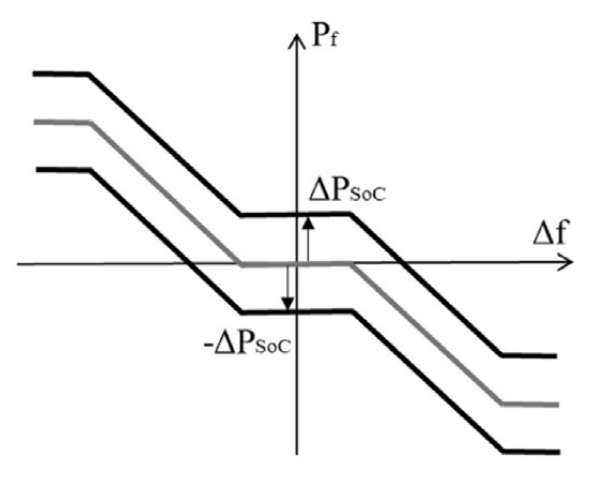
\includegraphics[width=6cm]{Abbildungen/DroopErweitert.png}
    \caption{SOC-Wiederherstellung mit Leistungssollwerten aus \parencite[]{noauthor_soc_nodate}}\label{Droopplus}
\end{figure}

\newpage
Abbildung~\ref{Droopplus} zeigt den resultierenden Leistungsverlauf.
Dabei muss die maximale Leistungsaufnahme bzw. -abgabe der Batterie berücksichtigt werden und die Vorgaben der
Übertragungsnetzbetreiber müssen eingehalten werden.
Ein sehr ähnlicher Ansatz wird auch in \parencite[]{mantar_gundogdu_battery_2018} für den EFR-Einsatz genutzt.
Dort wird allerdings noch einmal hervorgehoben, dass ein starrer Ziel-SOC von z.B. exakt 50 \% die 
Anzahl der Lade- bzw. Entladezyklen erhöht und sich damit negativ auf die Lebensdauer der Batterien auswirkt.
Für die praktische Umsetzung sollte also ein SOC-Bereich von z.B. 45 \% bis 55 \% angestrebt werden.
